\section{Results}
\label{sec:results}

\begin{figure}[t]
\centering
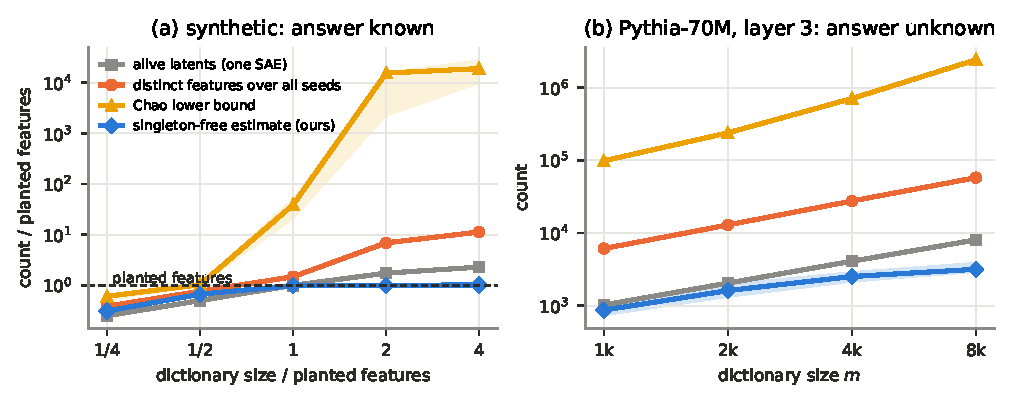
\includegraphics[width=\linewidth]{../figures/fig1_hero.pdf}
\caption{\textbf{Counting features with a fish-counting method.} (a) Synthetic activations with a known number $N$ of planted features (\SynFamilies{} settings; lines are medians, bands the range across settings). As the dictionary grows, the number of alive latents (gray) and the number of distinct features found across \SynSeeds{} seeds (orange) keep rising, and Chao's estimator (yellow) explodes. The singleton-free capture--recapture estimate (blue) rises until the dictionary is large enough and then levels off at the planted count (dashed). (b) The same quantities for Pythia-70M, where the true count is unknown. The blue band is the 95\% bootstrap interval.}
\label{fig:hero}
\end{figure}

\subsection{Naive counts overstate the number of features}
Table~\ref{tab:synth} and Figure~\ref{fig:hero}a compare every count and estimator with the planted number $N$. Once the dictionary has at least as many latents as there are planted features, every naive count is too high, and the error grows with the dictionary.
\begin{itemize}\setlength\itemsep{1pt}
\item \emph{Alive latents in one SAE:} \AliveRatioTwo$N$ at $m=2N$.
\item \emph{Distinct features across all seeds:} \UnionRatioEq$N$ at $m=N$ (median), and up to \UnionRatioMax$N$ at $m=4N$.
\item \emph{Equal-catchability estimators} (Lincoln--Petersen, $M_t$) and the Michaelis--Menten curve inherit the same inflation.
\item \emph{Heterogeneity estimators} built for exactly this kind of data are the worst. Chao's bound is $\ChaoRatioEq$ the truth at $m=N$ and up to $\ChaoRatioMax$ beyond, and the jackknife is also too high, increasingly so as the dictionary grows. The beta-binomial fitted to all species diverges in every setting.
\end{itemize}

\begin{table}[t]
\centering\small
\caption{\textbf{Estimated count divided by the planted count $N$} (median over settings; blind matching, $\tau=\MainTau$; \SynSeeds{} seeds). A superscript gives the number of settings in which the estimate diverged ($\hat N>10^9$), and ``div.'' means it diverged in every setting. The last two rows use the ground truth and are not available in practice. ``Reachable'' is the number of planted features that at least one seed caught.}
\label{tab:synth}
\begin{tabular}{lrrrrr}
\toprule
estimator & \multicolumn{5}{c}{dictionary size $m$} \\
 & $N/4$ & $N/2$ & $N$ & $2N$ & $4N$ \\
\midrule
alive latents (one SAE) & 0.25 & 0.50 & 1.00 & 1.74 & 2.28 \\
distinct features, all seeds & 0.38 & 0.76 & 1.47 & 6.88 & 11 \\
Michaelis--Menten asymptote & 0.40 & 0.80 & 1.49 & 18 & 46 \\
Lincoln--Petersen (Chapman) & 0.29 & 0.58 & 1.11 & 3.01 & 5.22 \\
Darroch $M_t$ & 0.38 & 0.76 & 1.47 & 8.02 & 16 \\
Chao $M_h$ bound & 0.61 & 1.03 & 39 & 15{,}470 & 18{,}962 \\
jackknife (2nd order) & 0.55 & 1.04 & 2.26 & 16 & 28 \\
beta-binomial, all species & div. & div. & div. & div. & div. \\
\quad singletons dropped, unbounded & 0.40$^{(3)}$ & 5.85$^{(3)}$ & 0.98 & div. & div. \\
two-class, singletons dropped, unbounded & 0.29 & 0.59 & 0.98 & 1.00$^{(1)}$ & 1.01 \\
\textbf{singleton-free (ours)} & 0.31 & 0.67 & 0.98 & 1.00 & 1.01 \\
singleton-free, oracle IDs & 0.28 & 0.67 & 1.00 & 1.00 & 1.00 \\
oracle: reachable (union, oracle IDs) & 0.31 & 0.71 & 1.00 & 1.00 & 1.00 \\
\bottomrule
\end{tabular}

\end{table}

\subsection{Why: junk latents are caught once}
Figure~\ref{fig:mechanism}a shows the capture frequencies behind these failures. Blind matching produces a spike of features caught by a single seed. At $m=N$, \JunkSingleEq{} of those singletons match no planted feature (median over settings), and at $m>N$ the figure is \JunkSingleOver. They are directions that one seed learned and no other seed reproduced, the analogue of sequencing-error ``species'' in microbial surveys \citep{chiu2016estimating}. Features seen by two or more seeds are almost all real: across frequency classes with at least 20 features, the largest junk fraction is \JunkMultiMax{} when $m\ge N$. Chao's bound grows with the square of the singleton count, which explains its explosion. Capture probabilities are also genuinely unequal (Figure~\ref{fig:mechanism}b). When the dictionary is too small, the rarest features are caught by few seeds or none, the heterogeneity that model $M_h$ describes \citep{otis1978statistical}.

\begin{figure}[t]
\centering
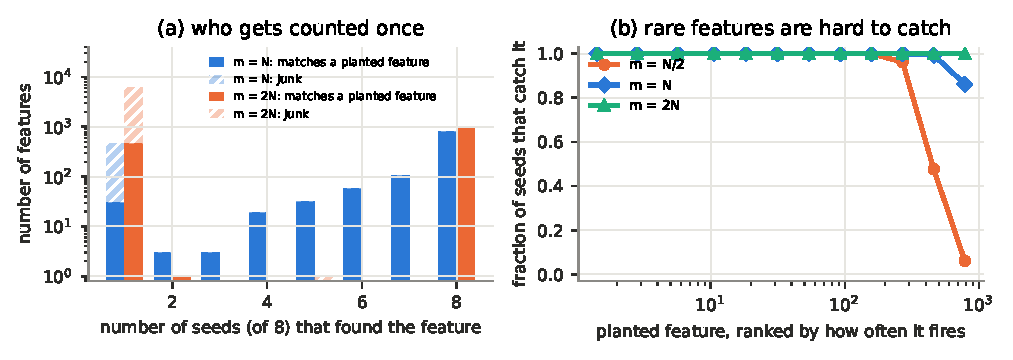
\includegraphics[width=\linewidth]{../figures/fig2_mechanism.pdf}
\caption{\textbf{Where naive counts go wrong} ($N=1024$, first data draw). (a) How many of the \SynSeeds{} seeds found each feature, under blind matching. Hatched bar segments match no planted feature. Almost all of them sit at ``found by one seed''. (b) Fraction of seeds that catch each planted feature (oracle matching), against how often the feature fires. With a dictionary half the needed size, rare features are seldom caught.}
\label{fig:mechanism}
\end{figure}

\subsection{The singleton-free estimate recovers the planted count}
\label{sec:sf}
Dropping the singletons and fitting a bounded catch-probability mixture to everything else removes the junk without discarding real features. Whenever $m\ge N$, the blind singleton-free estimate is within \SfMaxErrComplete{} of $N$ in all \NComplete{} settings, and it never diverges. It stays within \SfMaxErrCompleteTauLo{} and \SfMaxErrCompleteTauHi{} at matching thresholds $\tau=\TauLo$ and $\TauHi$, and within \SfMaxErrCompleteHalfPmin{} with half the probability floor ($p_{\min}=1/(2K)$). Doubling the dictionary from $m=N$ to $m=2N$ changes the estimate by a median factor of \PlateauMed{}: it has \emph{plateaued}.

When the dictionary is smaller than $N$, nothing can recover $N$. Even with oracle matching, only \OracleUnionQuarter{} ($m=N/4$) and \OracleUnionHalf{} ($m=N/2$) of planted features are ever caught by any of the \SynSeeds{} seeds. Here the estimate tracks the \emph{reachable} count: its ratio to the oracle union is \SfReachMed{} (median; range \SfReachLo--\SfReachHi). The estimate therefore behaves like a species-accumulation curve read in the dictionary-size direction. It rises while the dictionary is too small, and the height at which it stops rising is the feature count.

The two ablations isolate the two ingredients. Without the probability floor, the singleton-free beta-binomial diverges in most settings, often from a single stray recapture (Appendix~\ref{app:estimators}). With oracle matching, the same estimator is within a few percent of $N$ for $m\ge N$, so the remaining error comes from matching, not from the estimator.

\subsection{Predicting what more seeds will find}
\label{sec:heldout}
A population estimate makes a checkable prediction: train more seeds and you will find more of the population. We fit the singleton-free model on 4 of the 8 seeds (10 random subsets per setting) and predict how many features blind matching will find at least twice among all 8 (Figure~\ref{fig:heldout}).
\begin{itemize}\setlength\itemsep{1pt}
\item \emph{Dictionary smaller than the feature count.} New features keep appearing. Assuming no growth misses by \HeldSynSmallNoGrowthMed{} (median), and equal catchability by \HeldSynSmallMZeroMed. The singleton-free model misses by \HeldSynSmallSfMed{}, overshooting.
\item \emph{Dictionary at least as large as the feature count.} Four seeds already find almost everything. ``No growth'' is the right answer (median error \HeldSynBigNoGrowthMed), and the singleton-free model matches it in the median (\HeldSynBigSfMed) but overshoots by up to \HeldSynBigSfMax{} in the $m=N$ settings, where four seeds give it little to fit.
\end{itemize}
The estimator is thus useful for forecasting, but biased upward when fitted to few seeds.

\begin{figure}[t]
\centering
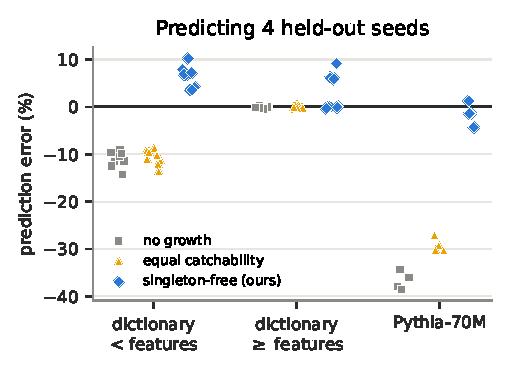
\includegraphics[width=0.55\linewidth]{../figures/fig3_heldout.pdf}
\caption{\textbf{Held-out seeds.} Error in predicting how many features 8 seeds will find at least twice, from 4 seeds. Each point is one setting, averaged over 10 random 4-seed subsets.}
\label{fig:heldout}
\end{figure}

\subsection{When features split}
\label{sec:hier}
Real features are hierarchical: a larger dictionary can replace one coarse feature with several finer ones \citep{bricken2023monosemanticity,leask2025sparse}. So what does the census count? We plant \HierParents{} parent features, each split into \HierC{} children, \HierChildren{} children in all. Whenever a parent is active, exactly one of its children fires. The children are therefore the features that generate the data, and a parent is their shared direction. Siblings have cosine \HierSiblingCos{} with each other and \HierParentCos{} with their parent, so at $\tau=\MainTau$ a latent can match a child or a parent but not both. We train \HierRuns{} SAEs (\SynSeeds{} seeds, $m$ from $N/8$ to $2N$ with $N$ the number of children, \HierDraws{} data draws, other settings unchanged). For the oracle we match latents against both levels (Figure~\ref{fig:hier}).

\begin{figure}[t]
\centering
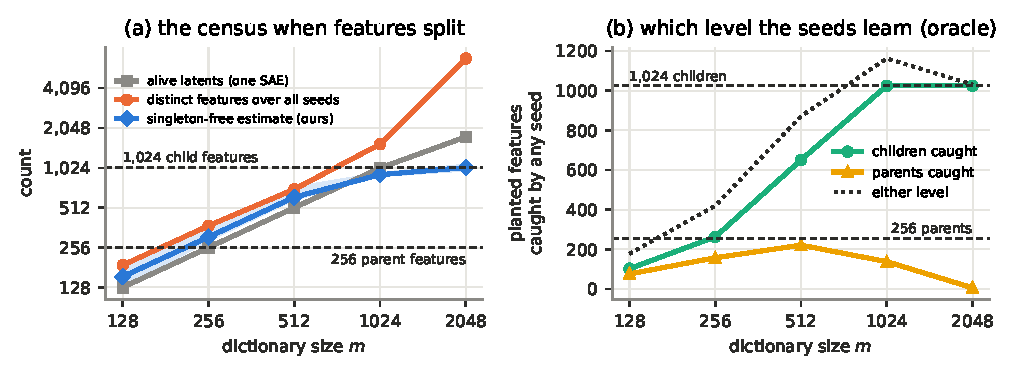
\includegraphics[width=\linewidth]{../figures/fig4_hierarchy.pdf}
\caption{\textbf{Features that split.} \HierParents{} planted parents, each with \HierC{} children (\HierChildren{} in all). (a) Counts against dictionary size, averaged over \HierDraws{} data draws; bands show the range over draws, and for the census the bootstrap intervals of both. The census rises with the dictionary and levels off at the child count only once there is room for every child. (b) Planted features caught by at least one of \SynSeeds{} seeds under oracle matching. Small dictionaries learn a mixture of parents and children.}
\label{fig:hier}
\end{figure}

\paragraph{Small dictionaries do not settle on the coarse level.} At $m=N/4$ there is room for exactly the \HierParents{} parents. Even so, the seeds learn a mixture: under oracle matching, \HierKidsQuarter{} children and \HierParsQuarter{} parents are caught by at least one seed. The census does not stop at \HierParents{}. It rises with the dictionary (\HierSfEighth, \HierSfQuarter{} and \HierSfHalf{} at $m=N/8$, $N/4$ and $N/2$), at \HierSfReachMed{} of the features reachable at either level (median; range \HierSfReachMin--\HierSfReachMax). A coarse level therefore does not create a false plateau.

\paragraph{Once the finest level fits, the census finds it.} At $m=2N$ the estimate is \HierSfDouble{} against \HierChildren{} children. It is within \HierSfErrDouble{} of the child count in both draws and at all three matching thresholds. Over the same seeds, the number of distinct latents reaches \HierUnionDouble{} (\HierUnionRatioMax-fold). For $m\ge N$, a median \HierJunkSingle{} of the features caught by only one seed match no planted feature at either level.

\paragraph{At $m=N$ the census undercounts.} The estimate is \HierSfFull{}, \HierSfErrFull{} below the child count, even though every child is caught by some seed. A likely cause is that the seeds disagree about the level: \HierParsFull{} parents are also caught by at least one seed. A child that only some seeds resolve looks rarer than it is. This setting is also the most sensitive to the threshold (\HierSfFullTauLo{} at $\tau=\TauLo$, \HierSfFullTauHi{} at $\tau=\TauHi$). At $\tau=\TauLo$ a parent latent can match a child latent, since their cosine of \HierParentCos{} clears the threshold. Held-out prediction is also worse with hierarchy. Fitted on four seeds, the singleton-free model overshoots the eight-seed count by a median of \HeldHierSmallSfMed{} for $m<N$ and \HeldHierBigSfMed{} (maximum \HeldHierBigSfMax) for $m\ge N$. ``No growth'' misses by \HeldHierSmallNoGrowthMed{} and \HeldHierBigNoGrowthMed{}.

Splitting changes how a census curve should be read, not whether the census works. At a given dictionary size, the census counts the features that size resolves, and a plateau marks the finest level the dictionaries can hold. On Pythia-70M the count keeps growing (\S\ref{sec:real}). Splitting produces the same growth whenever the finest level does not yet fit, so that growth alone does not show a fixed population larger than the dictionaries we trained.


\subsection{A census of Pythia-70M}
\label{sec:real}

We now count features where the answer is unknown: the residual stream after block \RealLayer{} of Pythia-70M, with \RealSeeds{} seeds at each of four dictionary sizes (Table~\ref{tab:real}, Figure~\ref{fig:hero}b).

\begin{table}[t]
\centering\small
\caption{\textbf{Census of Pythia-70M} (layer \RealLayer, \RealSeeds{} seeds per size, $\tau=\MainTau$). FVU is the fraction of variance unexplained on held-out tokens (mean over seeds). ``Distinct, all seeds'' is the union over seeds. ``Seen $\ge2$'' counts features reproduced by at least two seeds. The interval is a 95\% bootstrap interval for the singleton-free estimate.}
\label{tab:real}
\begin{tabular}{rrrrrrrl}
\toprule
$m$ & FVU & alive & distinct, all seeds & seen $\ge 2$ & Chao $M_h$ & singleton-free & 95\% CI \\
\midrule
1{,}024 & 0.090 & 1{,}024 & 6{,}107 & 543 & 98{,}244 & 870 & [728, 1{,}083] \\
2{,}048 & 0.082 & 2{,}048 & 12{,}900 & 934 & 238{,}236 & 1{,}616 & [1{,}303, 2{,}011] \\
4{,}096 & 0.077 & 4{,}089 & 27{,}515 & 1{,}428 & 705{,}721 & 2{,}520 & [2{,}113, 2{,}941] \\
8{,}192 & 0.073 & 8{,}044 & 57{,}614 & 1{,}867 & 2{,}405{,}854 & 3{,}172 & [2{,}869, 3{,}952] \\
\bottomrule
\end{tabular}

\end{table}

\paragraph{Seeds disagree much more than on planted features.} At $m=8192$, \RealSingleFrac{} of the distinct features found across seeds were found by one seed only, and just \RealAllSeedsEight{} by all eight. The union over seeds grows \RealUnionGrowth-fold from $m=1024$ to $m=8192$, slightly faster than the dictionary itself, and Chao's bound reaches the millions. Both are the junk-driven signatures of the synthetic over-complete regime.

\paragraph{The singleton-free census.} The estimated number of reproducible features grows from \RealSfOne{} (95\% CI \RealSfLoOne--\RealSfHiOne) at $m=1024$ to \RealSfEight{} (\RealSfLoEight--\RealSfHiEight) at $m=8192$. Each doubling of the dictionary multiplies the estimate by \RealGrowthOne, \RealGrowthTwo{} and \RealGrowthFour{}. Growth is slowing, but by the logic of \S\ref{sec:sf} it has not stopped, so these dictionaries have not yet reached the plateau and \RealSfEight{} is a lower bound for this layer under our training budget. At $m=8192$ only about \RealReproFrac{} of a single SAE's alive latents correspond to reproducible features, a regime we did not see with planted features.

\paragraph{Held-out seeds confirm the forecasts.} Fitted on 4 seeds, the singleton-free model predicts how many features all 8 seeds reproduce to within \HeldRealSfMax{} at every dictionary size (median \HeldRealSfMed; Figure~\ref{fig:heldout}). In the median, assuming no new features would appear misses by \HeldRealNoGrowthMed, and assuming equal catchability by \HeldRealMZeroMed. This test needs no ground truth, so it is the strongest evidence that the census describes real structure in the seeds' agreement.

\paragraph{What the census is sensitive to.} The matching threshold matters more for real features than for planted ones (Appendix Table~\ref{tab:real_tau}). At $m=8192$ the estimate is \RealSfEightTauLo{} at $\tau=\TauLo$ and \RealSfEightTauHi{} at $\tau=\TauHi$. The growth with dictionary size holds for $\tau\le\MainTau$, but at $\tau=\TauHi$ the estimate falls between $m=4096$ and $m=8192$. Real features are reproduced less exactly than planted directions, so deciding when two latents are ``the same feature'' is a modelling choice that the count inherits. The number of seeds matters less: at $m=8192$, fitting 4, 6 and 8 seeds gives \RealSfEightKFour, \RealSfEightKSix{} and \RealSfEight.

\paragraph{More training data makes seeds agree, and raises the count.} We retrained the $m=2048$ family on \RealLongTokens{} tokens, five times more data, in one pass (\RealLongStepRatio{} times as many training steps). The model, layer and evaluation set are unchanged. The new SAEs reconstruct better (FVU \RealLongFvu{} vs \RealFvuTwo) and agree more: \RealLongAllSeeds{} features are found by all eight seeds, against \RealAllSeedsTwo. The singleton-free estimate rises from \RealSfTwo{} to \RealLongSf{} (95\% CI \RealLongSfLo--\RealLongSfHi), a factor of \RealLongRatio. Across the three matching thresholds it now ranges only from \RealLongTauMin{} to \RealLongTauMax, against \RealTwoTauMin{} to \RealTwoTauMax{} before, and the held-out prediction from four seeds is off by \RealLongHeldErr. Part of the seed disagreement on Pythia is therefore a training-budget effect. Our census counts are lower bounds in two senses: the dictionaries are too small to plateau, and more training would reveal more reproducible features.


